\documentclass[11pt,a4paper]{article}

\usepackage[margin=1in]{geometry}
\usepackage[T1]{fontenc}
\usepackage[utf8]{inputenc}
\usepackage{lmodern}
\usepackage{amsmath,amssymb}
\usepackage{array}
\usepackage{booktabs}
\usepackage{float}
\usepackage{graphicx}
\usepackage{hyperref}
\usepackage{longtable}
\usepackage{tabularx}
\usepackage{xcolor}
\usepackage{enumitem}

\graphicspath{{../End-to-end/}{../}}
\hypersetup{
  colorlinks=true,
  linkcolor=blue!50!black,
  citecolor=blue!50!black,
  urlcolor=blue!50!black
}

\setlength{\parindent}{0pt}
\setlength{\parskip}{0.45em}
\renewcommand{\arraystretch}{1.15}

\newcommand{\ones}{\mathbf{1}}
\newcommand{\diag}{\operatorname{diag}}

\begin{document}
\hypersetup{pageanchor=false}

\begin{titlepage}
\centering
{\Large MSc AI Lab Project Report\par}
\vspace{1.2cm}
{\huge\bfseries End-to-End Portfolio Optimization with CNN-GARCH and RIENet\par}
\vspace{1cm}
{\large Wacil Lakbir \\ Sneha Basker\par}
\vspace{0.6cm}
{\large Supervisor: Christian Bongiorno\par}
\vspace{0.4cm}
{\normalsize
Emails: \texttt{[add-wacil-email]} \quad | \quad \texttt{[add-sneha-email]}\par
}
\vspace{0.25cm}
{\normalsize Git repository (maintainer access): \texttt{[add-maintainer-git-link]}\par}
\vspace{0.25cm}
{\normalsize Date: April 9, 2026\par}
\vfill

\begin{minipage}{0.92\textwidth}
\textbf{Abstract.}
This project studies global minimum variance (GMV) portfolio construction under noisy covariance estimation. The practical difficulty is not the optimizer itself, but the quality of the covariance matrix given to the optimizer. We therefore compare three levels of modeling: a benchmark GARCH pipeline, a hybrid CNN-GARCH model for marginal volatility forecasting, and a cleaned covariance pipeline that combines the neural volatility model with a RIENet-style rotation-invariant correlation cleaning step. The empirical study is based on cleaned WIKI adjusted-price data from January 4, 2000 to March 27, 2018, with a 90-day rolling window and a train/test split at October 4, 2012. The main result comes from the 50-stock unconstrained GMV experiment: GMV-NN-Clean achieves the lowest annualized volatility (12.75\%), while GMV-NN delivers the highest Sharpe ratio (1.4190). Additional constrained and Monte Carlo experiments confirm that the neural volatility model is competitive against standard GARCH baselines and often improves out-of-sample risk-adjusted performance. The report positions these results relative to classical GARCH, covariance-cleaning methods, and recent hybrid neural-volatility literature, then discusses remaining limitations such as transaction costs, turnover, and sensitivity to market regime changes.
\end{minipage}
\vfill
\end{titlepage}
\clearpage
\pagenumbering{arabic}
\hypersetup{pageanchor=true}

\section{Introduction}

Minimum-variance portfolio construction is one of the cleanest settings in quantitative finance because the optimization target is explicit: reduce realized portfolio risk while maintaining acceptable diversification. In practice, however, the global minimum variance portfolio is only as good as the covariance matrix that enters the optimizer. Small errors in estimated volatilities or correlations are amplified when the covariance matrix is inverted, which can produce unstable weights, concentration, and disappointing out-of-sample behavior.

This estimation problem motivates our project. Rather than changing the downstream optimizer, we keep the GMV rule fixed and focus on improving the upstream covariance-estimation pipeline. The first reason to consider GARCH is financial interpretability. Daily returns exhibit volatility clustering, persistence, and heteroskedasticity, and the GARCH family was designed precisely to model these stylized facts \cite{engle1982,bollerslev1986}. GARCH(1,1) remains a strong benchmark because it is parsimonious, stable, and easy to deploy on rolling windows. At the same time, pure GARCH imposes a rigid functional form and treats each asset through a small set of linear lag interactions.

Our response is a hybrid architecture. A convolutional neural network reads a 90-day return window and learns richer nonlinear temporal features than a plain handcrafted recursion. Instead of discarding econometric structure, we map the neural output into a stable GARCH-like parameterization, which preserves interpretability and imposes sensible constraints on volatility dynamics. This gives a CNN-GARCH model that aims to be more flexible than classical GARCH without becoming a black-box forecaster.

Marginal volatilities alone do not solve the GMV problem. Portfolio variance also depends on cross-asset dependence, and empirical rolling correlations are notoriously noisy in high dimension. This is why the project adds a RIENet-style covariance cleaning block inspired by rotation-invariant estimation \cite{ledoit2004,bongiorno2025e2e}. The idea is to regularize the eigenspectrum of the correlation matrix before building the covariance matrix used by the optimizer.

The report addresses the following research question: can a hybrid CNN-GARCH volatility model, combined with correlation cleaning, improve out-of-sample GMV behavior relative to a benchmark GARCH pipeline? Our answer is nuanced. The experiments show clear improvements in several settings, especially for volatility reduction in the 50-stock unconstrained GMV setup, but they do not prove that the problem is definitively solved in every market regime or portfolio constraint set.

The main contributions of the project are the following:
\begin{itemize}[leftmargin=1.5em]
\item a benchmark comparison between classical GARCH, hybrid CNN-GARCH, and CNN-GARCH plus RIENet-style cleaning in a common GMV framework;
\item a stable neural parameterization of GARCH coefficients through the triplet $(\omega, C, \rho)$;
\item an end-to-end experimental pipeline that connects synthetic pretraining, real-data fine-tuning, covariance construction, and portfolio evaluation;
\item a numerical study covering the main unconstrained result, constrained portfolio variants, and Monte Carlo robustness tests.
\end{itemize}

\section{State of the Art}

\subsection{From Markowitz to covariance regularization}

Modern portfolio theory starts from the mean-variance framework of Markowitz \cite{markowitz1952}. In the GMV special case, the expected-return vector does not need to be forecast explicitly; the main object is the covariance matrix. This simplification is powerful, but it also exposes the central weakness of the method: sample covariance estimates can be unstable, especially when the number of assets is large relative to the available lookback window. Ledoit and Wolf \cite{ledoit2004} showed that shrinkage and conditioning are natural ways to reduce estimation noise and improve out-of-sample performance.

The Bongiorno end-to-end paper used in this project pushes this logic further by combining portfolio optimization with rotation-invariant covariance cleaning \cite{bongiorno2025e2e}. In that line of work, the relevant question is no longer only how to estimate covariance in isolation, but how to estimate it in a way that directly helps the downstream variance-minimization objective.

\subsection{Why GARCH remains a strong baseline}

ARCH and GARCH were introduced to model time-varying conditional variance in financial returns \cite{engle1982,bollerslev1986}. They remain the canonical baseline for volatility forecasting because they capture volatility clustering with very few parameters. For daily equities, this is a sensible starting point: a one-step recursion is computationally manageable, interpretable, and aligned with rolling risk management.

For our project, GARCH is important for two reasons. First, it gives a benchmark that is financially grounded rather than purely machine-learning-based. Second, it suggests a useful inductive bias: even if a neural model learns latent features from return windows, the final variance forecast can still be constrained to behave like a stable GARCH recursion.

\subsection{Neural and hybrid volatility forecasting}

Recent literature increasingly combines econometric structure with neural sequence models instead of choosing one family against the other. Micha\'nk\'ow, Kwiatkowski, and Morajda propose hybrid GRU-GARCH models for volatility and risk forecasting and report improved point forecasts on several assets \cite{michankow2023}. Wang et al.\ develop a deep-learning-enhanced multivariate GARCH model in which recurrent neural components enrich a BEKK-style volatility structure \cite{wang2025}. The common message is that hybridization can improve nonlinear feature extraction while retaining some interpretability and structure from classical volatility models.

Our project belongs to this hybrid family, but with a different design choice. Instead of a recurrent architecture, we use a compact stack of dilated one-dimensional convolutions. The practical reason is that dilated convolutions can summarize multi-scale lag information efficiently, with a small parameter budget and parallelizable computation. The model then projects the learned representation back into a GARCH-like parameter space.

\subsection{Positioning of the present work}

The second Bongiorno paper relevant to this project focuses on end-to-end variance minimization and leverage resilience under a compact neural architecture \cite{bongiorno2025icaif}. Our work is closely aligned with that view of portfolio optimization as a full pipeline problem: forecasting, covariance cleaning, and portfolio construction should be evaluated together. The present project therefore sits at the intersection of three strands: classical heteroskedastic modeling, neural volatility forecasting, and covariance cleaning for portfolio optimization.

\section{Problem Formulation and Data}

\subsection{Data source and cleaning}

The empirical dataset is built from WIKI adjusted prices. The cleaning and filtering logic is implemented in \texttt{data\_stocks\_WIKI\_price.py}. The retained period runs from January 4, 2000 to March 27, 2018, for a final cleaned universe of 1338 stocks over 4585 trading days.

The main data filters are the following:
\begin{itemize}[leftmargin=1.5em]
\item rows with zero trading volume are removed before return construction;
\item returns are computed from adjusted close prices;
\item only assets with sufficiently complete usable histories are kept;
\item assets priced below 3 USD on the first test date are excluded;
\item assets with more than 20 consecutive zero returns are removed in order to reduce stale-price effects.
\end{itemize}

The temporal split used throughout the project is:
\begin{itemize}[leftmargin=1.5em]
\item training period: January 4, 2000 to October 3, 2012;
\item test period: October 4, 2012 to March 27, 2018.
\end{itemize}

All rolling experiments use a lookback window of $W=90$ trading days.

\subsection{Notation and portfolio objective}

Let $r_{i,t}$ denote the daily return of asset $i$ at day $t$, and let
\[
x_{i,t} = \left(r_{i,t-W+1}, \dots, r_{i,t}\right) \in \mathbb{R}^{W}
\]
be the 90-day input window used to forecast one-step-ahead conditional variance. Let $\hat{\sigma}_{i,t+1}^2$ denote the forecast variance for asset $i$, and define the diagonal volatility matrix
\[
D_t = \diag(\hat{\sigma}_{1,t}, \dots, \hat{\sigma}_{N,t}).
\]
Let $C_t$ denote the rolling correlation matrix, or its cleaned counterpart when a covariance cleaner is applied. The portfolio covariance estimate is then
\[
\Sigma_t = D_t C_t D_t.
\]

For the unconstrained GMV problem, the portfolio weights solve
\[
w_t^\star = \frac{\Sigma_t^{-1}\ones}{\ones^\top \Sigma_t^{-1}\ones}.
\]
This formula highlights why covariance quality is crucial: any instability in $\Sigma_t$ is directly transferred to the weights through matrix inversion.

In some experiments, weight constraints are added, such as per-asset caps or practical long-only restrictions. These variants do not change the conceptual point of the project. They only modify the optimizer; the central challenge remains the same, namely producing a covariance estimate that is sufficiently stable and predictive for out-of-sample risk control.

\section{Methodology}

\subsection{Synthetic pretraining}

The project first pretrains the volatility network on synthetic GARCH(1,1) series before adapting it to real equity data. The exploratory setup recovered from \texttt{Main.ipynb} uses 2000 simulated series, 2000 samples, a 90-day input window, and a 60/20/20 split between training, validation, and test subsets. This stage is not meant to replace real-data learning. Its role is to initialize the model on generic heteroskedastic dynamics so that fine-tuning on equities starts from a financially meaningful prior rather than from random weights.

\subsection{Real-data fine-tuning}

Real-data training is handled in \texttt{test\_on\_real\_time\_series.ipynb}. The final fine-tuning configuration uses a 90-day window, about 20 epochs, a learning rate around $10^{-4}$, weight decay around $10^{-6}$, validation-based checkpoint selection, and zero-aware filtering. The preprocessing also imposes a cap on the fraction of zero returns and a small floor on the variance proxy in order to avoid degenerate log-loss behavior on illiquid or nearly constant series.

The training loss is an MSE on log-variance targets:
\[
\mathcal{L}_{\mathrm{vol}}
=
\frac{1}{M}\sum_{m=1}^{M}
\left[
\log\left(\hat{\sigma}_{m}^2 + \varepsilon\right)
-
\log\left(y_{m} + \varepsilon\right)
\right]^2,
\]
where $y_m$ is a next-day realized variance proxy derived from squared returns and $\varepsilon$ is a small numerical floor. The notebooks report a strong improvement after the zero-aware fine-tuning stage, which is consistent with the idea that noisy or stale observations can distort volatility targets on daily equity data.

\subsection{Hybrid CNN-GARCH architecture}

The core model is implemented in \texttt{model.py}. Each input window is passed through five dilated one-dimensional convolutional layers with kernel size 3 and dilation rates $(1,2,4,8,16)$. Each block is followed by GroupNorm and LeakyReLU before a dense prediction head produces the parameters of the final variance recursion. The model used in the main portfolio notebooks contains 14{,}499 trainable parameters.

The choice of five layers is deliberate. With kernel size 3 and exponentially increasing dilations, the receptive field reaches 63 days, which is large enough to capture medium-term volatility persistence while keeping the architecture compact. The 90-day window is still summarized globally by the final stacked representation, so the network can combine recent shocks with longer-range volatility context.

Instead of predicting the usual GARCH coefficients directly, the network outputs a stable triplet $(\omega, C, \rho)$ and converts it into
\[
\alpha = C\rho, \qquad \beta = C(1-\rho).
\]
When $0 < C < 1$ and $0 < \rho < 1$, this construction ensures
\[
\alpha + \beta = C < 1,
\]
which enforces a stable GARCH-like recursion. The one-step variance update is
\[
\hat{\sigma}_{i,t+1}^2
=
\omega_{i,t}
+
\alpha_{i,t} r_{i,t}^2
+
\beta_{i,t}\hat{\sigma}_{i,t}^2.
\]
This is one of the main design strengths of the project: the neural network learns nonlinear temporal features, but the final output remains financially interpretable and structurally close to GARCH.

\subsection{RIENet-style correlation cleaning}

Even with accurate marginal volatilities, GMV portfolios remain sensitive to noise in the correlation matrix. The covariance-cleaning part of the project therefore follows the logic of rotation-invariant estimation emphasized in \cite{ledoit2004,bongiorno2025e2e}. Let $S_t$ be a rolling sample correlation matrix with spectral decomposition
\[
S_t = V_t \Lambda_t V_t^\top.
\]
The cleaner regularizes the eigenvalue structure while preserving the eigenvector basis, producing
\[
\widetilde{C}_t = V_t \widetilde{\Lambda}_t V_t^\top.
\]
The cleaned covariance matrix is then
\[
\widetilde{\Sigma}_t = D_t \widetilde{C}_t D_t.
\]

The project compares three portfolio pipelines:
\begin{itemize}[leftmargin=1.5em]
\item \textbf{GMV-GARCH}: benchmark volatility recursion with standard correlation input;
\item \textbf{GMV-NN}: hybrid CNN-GARCH volatility with standard correlation input;
\item \textbf{GMV-NN-Clean}: hybrid CNN-GARCH volatility combined with cleaned correlations.
\end{itemize}

\subsection{Pseudo-code}

\textbf{Training pipeline}
\begin{enumerate}[leftmargin=1.5em]
\item Simulate synthetic GARCH series and pretrain the CNN-GARCH model on one-step variance prediction.
\item Build the cleaned real-equity panel and extract rolling 90-day windows.
\item Fine-tune the model on real data with zero-aware filtering and checkpoint on validation loss.
\item Save the best neural volatility model and reuse it in the portfolio notebooks.
\end{enumerate}

\textbf{Daily portfolio construction pipeline}
\begin{enumerate}[leftmargin=1.5em]
\item For each rebalancing date, compute rolling returns on the selected stock universe.
\item Predict asset-wise marginal volatilities with either GARCH or CNN-GARCH.
\item Estimate the rolling correlation matrix and optionally apply RIENet-style cleaning.
\item Assemble the covariance estimate $\Sigma_t = D_t C_t D_t$.
\item Solve the GMV optimization problem and record out-of-sample returns.
\end{enumerate}

\section{Numerical Results}

\subsection{Experimental setup}

The main portfolio results are produced in the \texttt{End-to-end} notebooks. The user-specified primary result is the 50-stock unconstrained experiment from \path{portfolio_unconstrained_rienet.ipynb}. Supporting results come from the constrained 30-stock and 100-stock experiments in \path{portfolio_optimization_rienet.ipynb} and \path{portfolio_optimization.ipynb}. A separate Monte Carlo study in \path{Portfolio.ipynb} repeatedly samples 30-stock universes to test robustness.

The evaluation logic is simple. For GMV portfolios, the first objective is lower realized volatility. When two methods have comparable volatility, the second criterion is the Sharpe ratio. This is consistent with the core purpose of minimum-variance allocation.

\subsection{Main result: 50-stock unconstrained GMV}

Table \ref{tab:main-unconstrained} contains the main result emphasized in this report.

\begin{table}[H]
\centering
\caption{Main result from \texttt{portfolio\_unconstrained\_rienet.ipynb}.}
\label{tab:main-unconstrained}
\begin{tabular}{lccc}
\toprule
Method & Ann. Return (\%) & Ann. Vol (\%) & Sharpe \\
\midrule
GMV-GARCH & 17.39 & 13.95 & 1.2468 \\
GMV-NN & 20.43 & 14.40 & 1.4190 \\
GMV-NN-Clean & 17.53 & 12.75 & 1.3755 \\
\bottomrule
\end{tabular}
\end{table}

Two conclusions matter. First, the cleaned neural pipeline produces the lowest portfolio volatility, which is the primary objective of GMV. Second, the uncleaned neural variant delivers the highest Sharpe ratio. This means the project does not yield a single uniformly dominant model across all metrics, but it does show that the neural volatility model and the cleaning stage both create measurable value.

\begin{figure}[H]
\centering
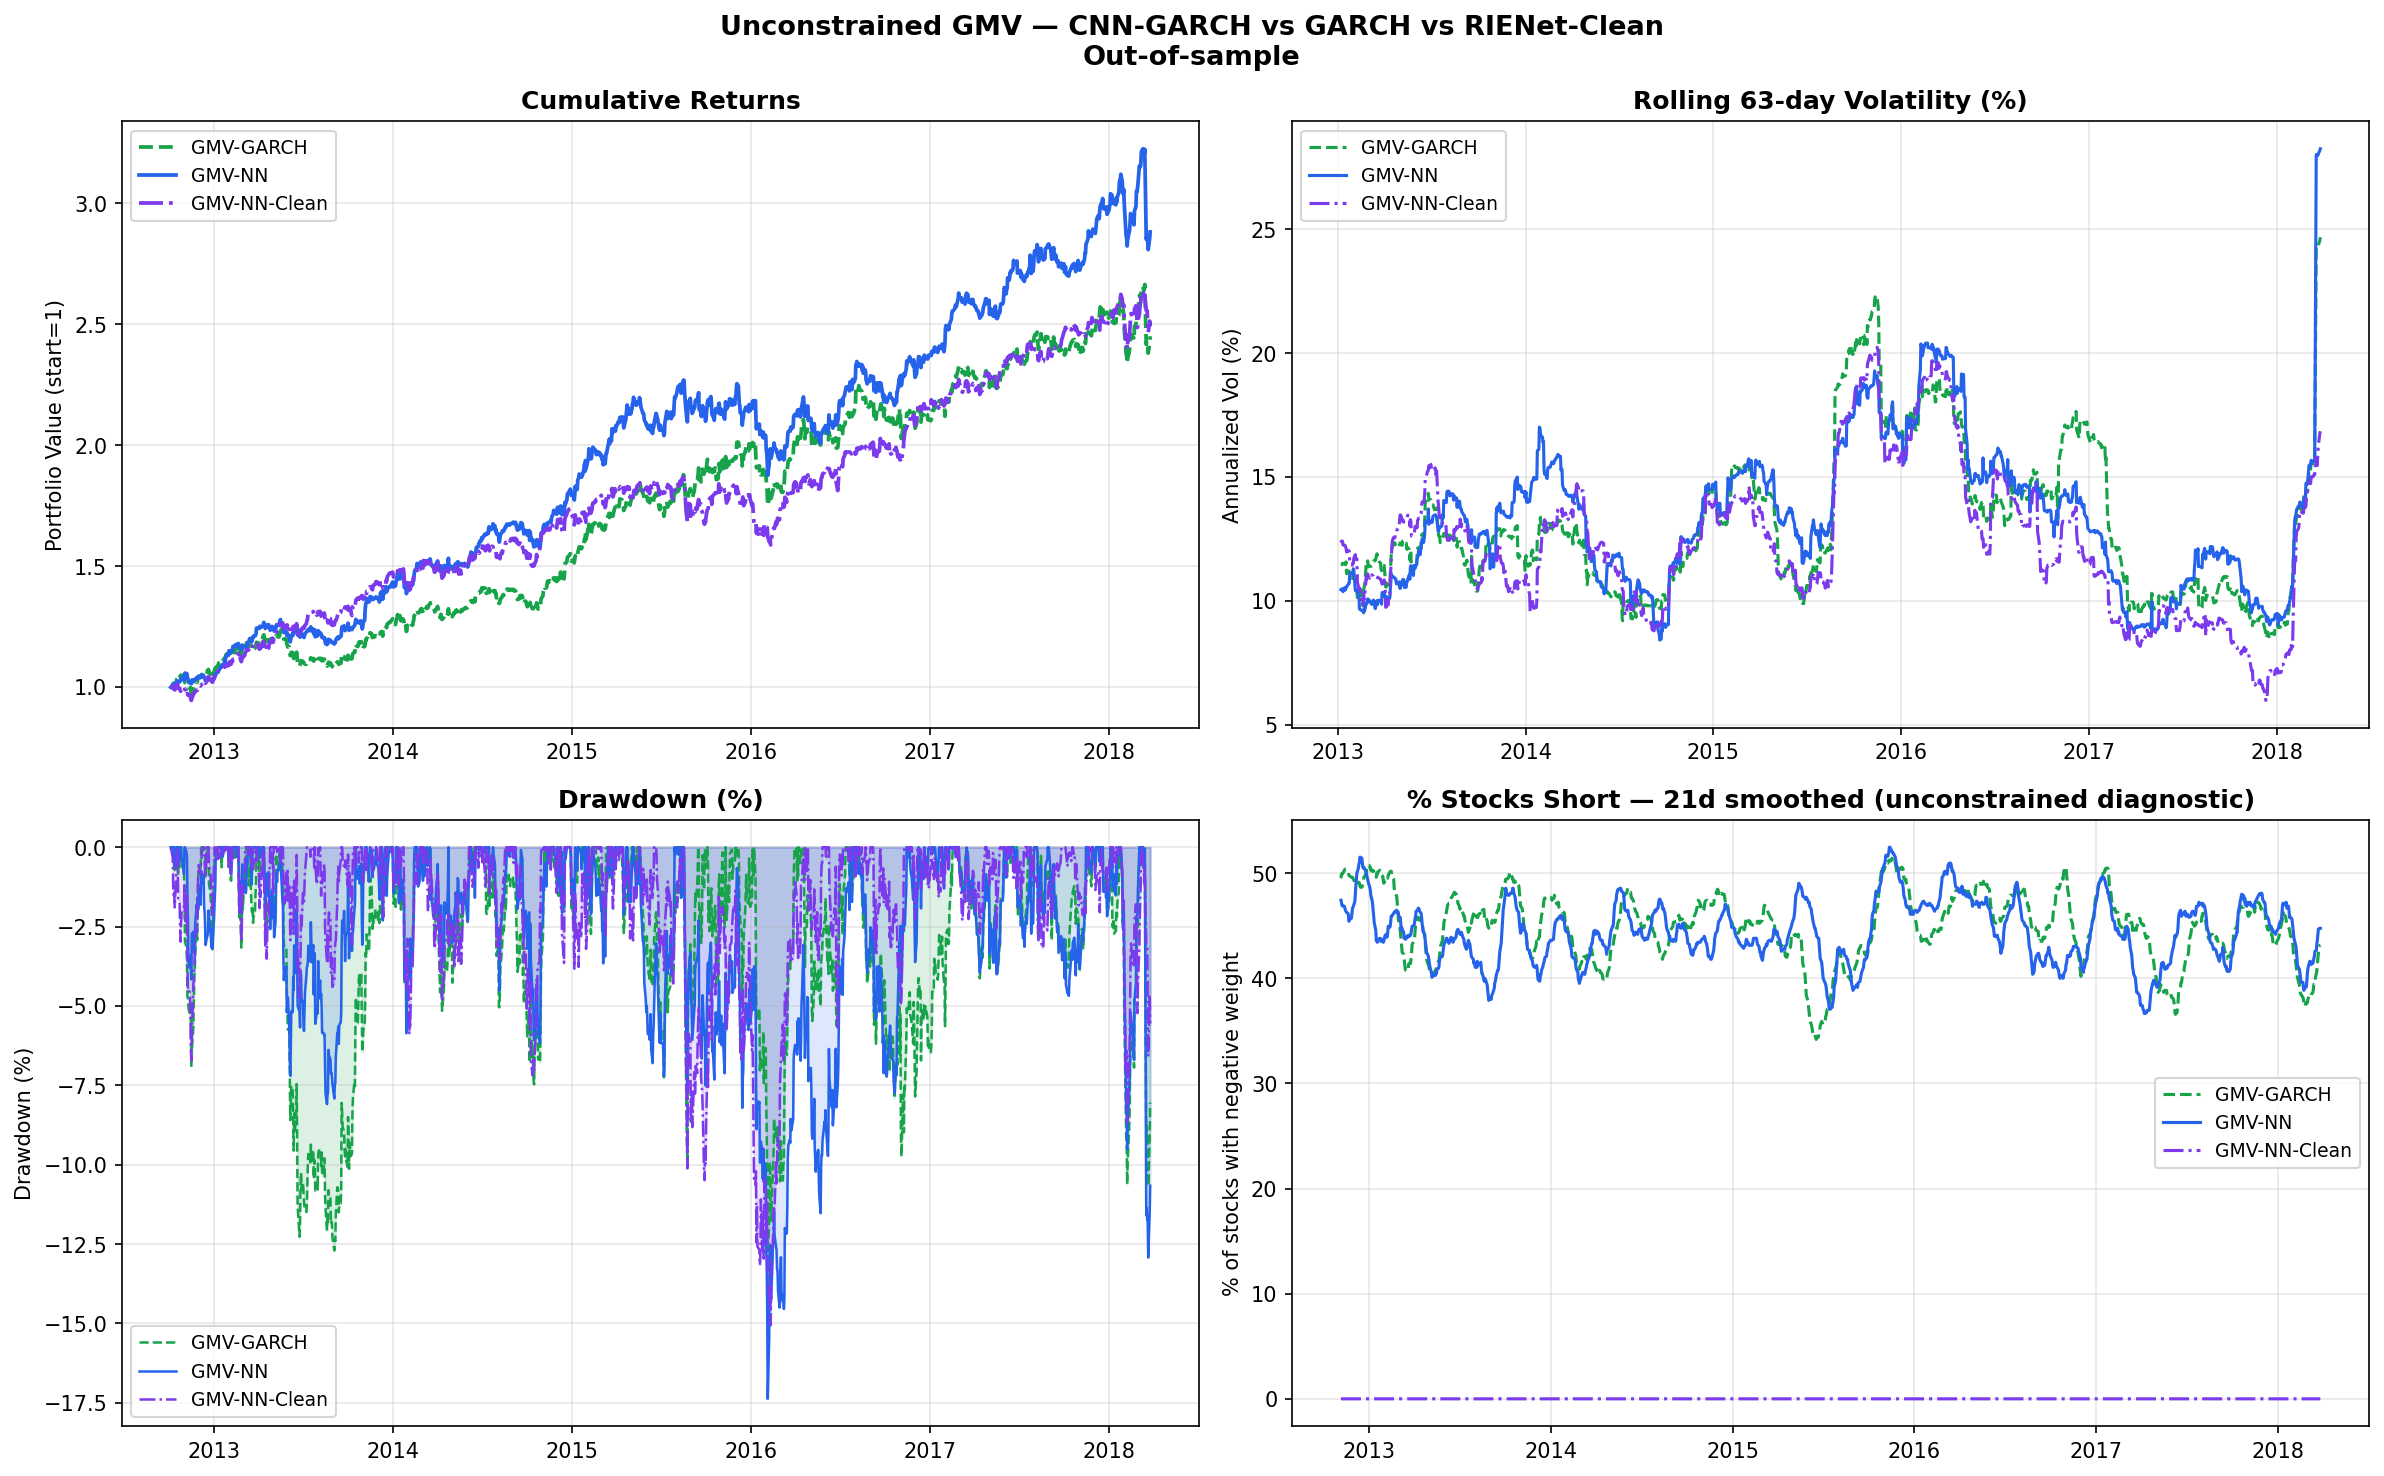
\includegraphics[width=0.82\textwidth]{gmv_unconstrained_results.png}
\caption{Cumulative performance comparison for the 50-stock unconstrained GMV experiment.}
\label{fig:gmv-unconstrained}
\end{figure}

\subsection{Supporting results: constrained GMV experiments}

The constrained 30-stock experiment also shows a strong neural baseline.

\begin{table}[H]
\centering
\caption{Constrained 30-stock result from \texttt{portfolio\_optimization\_rienet.ipynb}.}
\label{tab:constrained-30}
\begin{tabular}{lccc}
\toprule
Method & Ann. Return (\%) & Ann. Vol (\%) & Sharpe \\
\midrule
GMV-GARCH & 16.73 & 11.45 & 1.4613 \\
GMV-NN & 19.19 & 11.44 & 1.6781 \\
GMV-NN-Clean & 19.22 & 13.02 & 1.4756 \\
\bottomrule
\end{tabular}
\end{table}

Here the plain neural volatility model dominates on Sharpe while matching or slightly improving volatility relative to the benchmark. The cleaned variant does not dominate in this constrained setting, which is important for an honest interpretation: covariance cleaning helps in some configurations more clearly than in others.

\begin{table}[H]
\centering
\caption{Summary of the 100-stock constrained comparison from \texttt{portfolio\_optimization.ipynb}.}
\label{tab:constrained-100}
\begin{tabular}{lcccc}
\toprule
Method & Return (\%) & Vol (\%) & Sharpe & Calmar \\
\midrule
Equal-Weight & 17.26 & 14.33 & 1.2044 & 1.0647 \\
Inv-Var NN & 17.53 & 12.15 & 1.4422 & 1.3357 \\
GMV-GARCH & 16.05 & 10.92 & 1.4697 & 1.3698 \\
GMV-NN & 18.39 & 10.86 & 1.6939 & 1.7504 \\
GMV-GARCH-Clean & 16.27 & 12.12 & 1.3421 & 1.2959 \\
GMV-NN-Clean & 17.48 & 12.22 & 1.4305 & 1.3247 \\
\bottomrule
\end{tabular}
\end{table}

This larger experiment reinforces the main message: the neural volatility block is competitive and can materially improve the portfolio pipeline. At the same time, the effect of cleaning is not universally monotone across all constrained settings, so the report should avoid claiming that the problem is completely solved.

\begin{figure}[H]
\centering
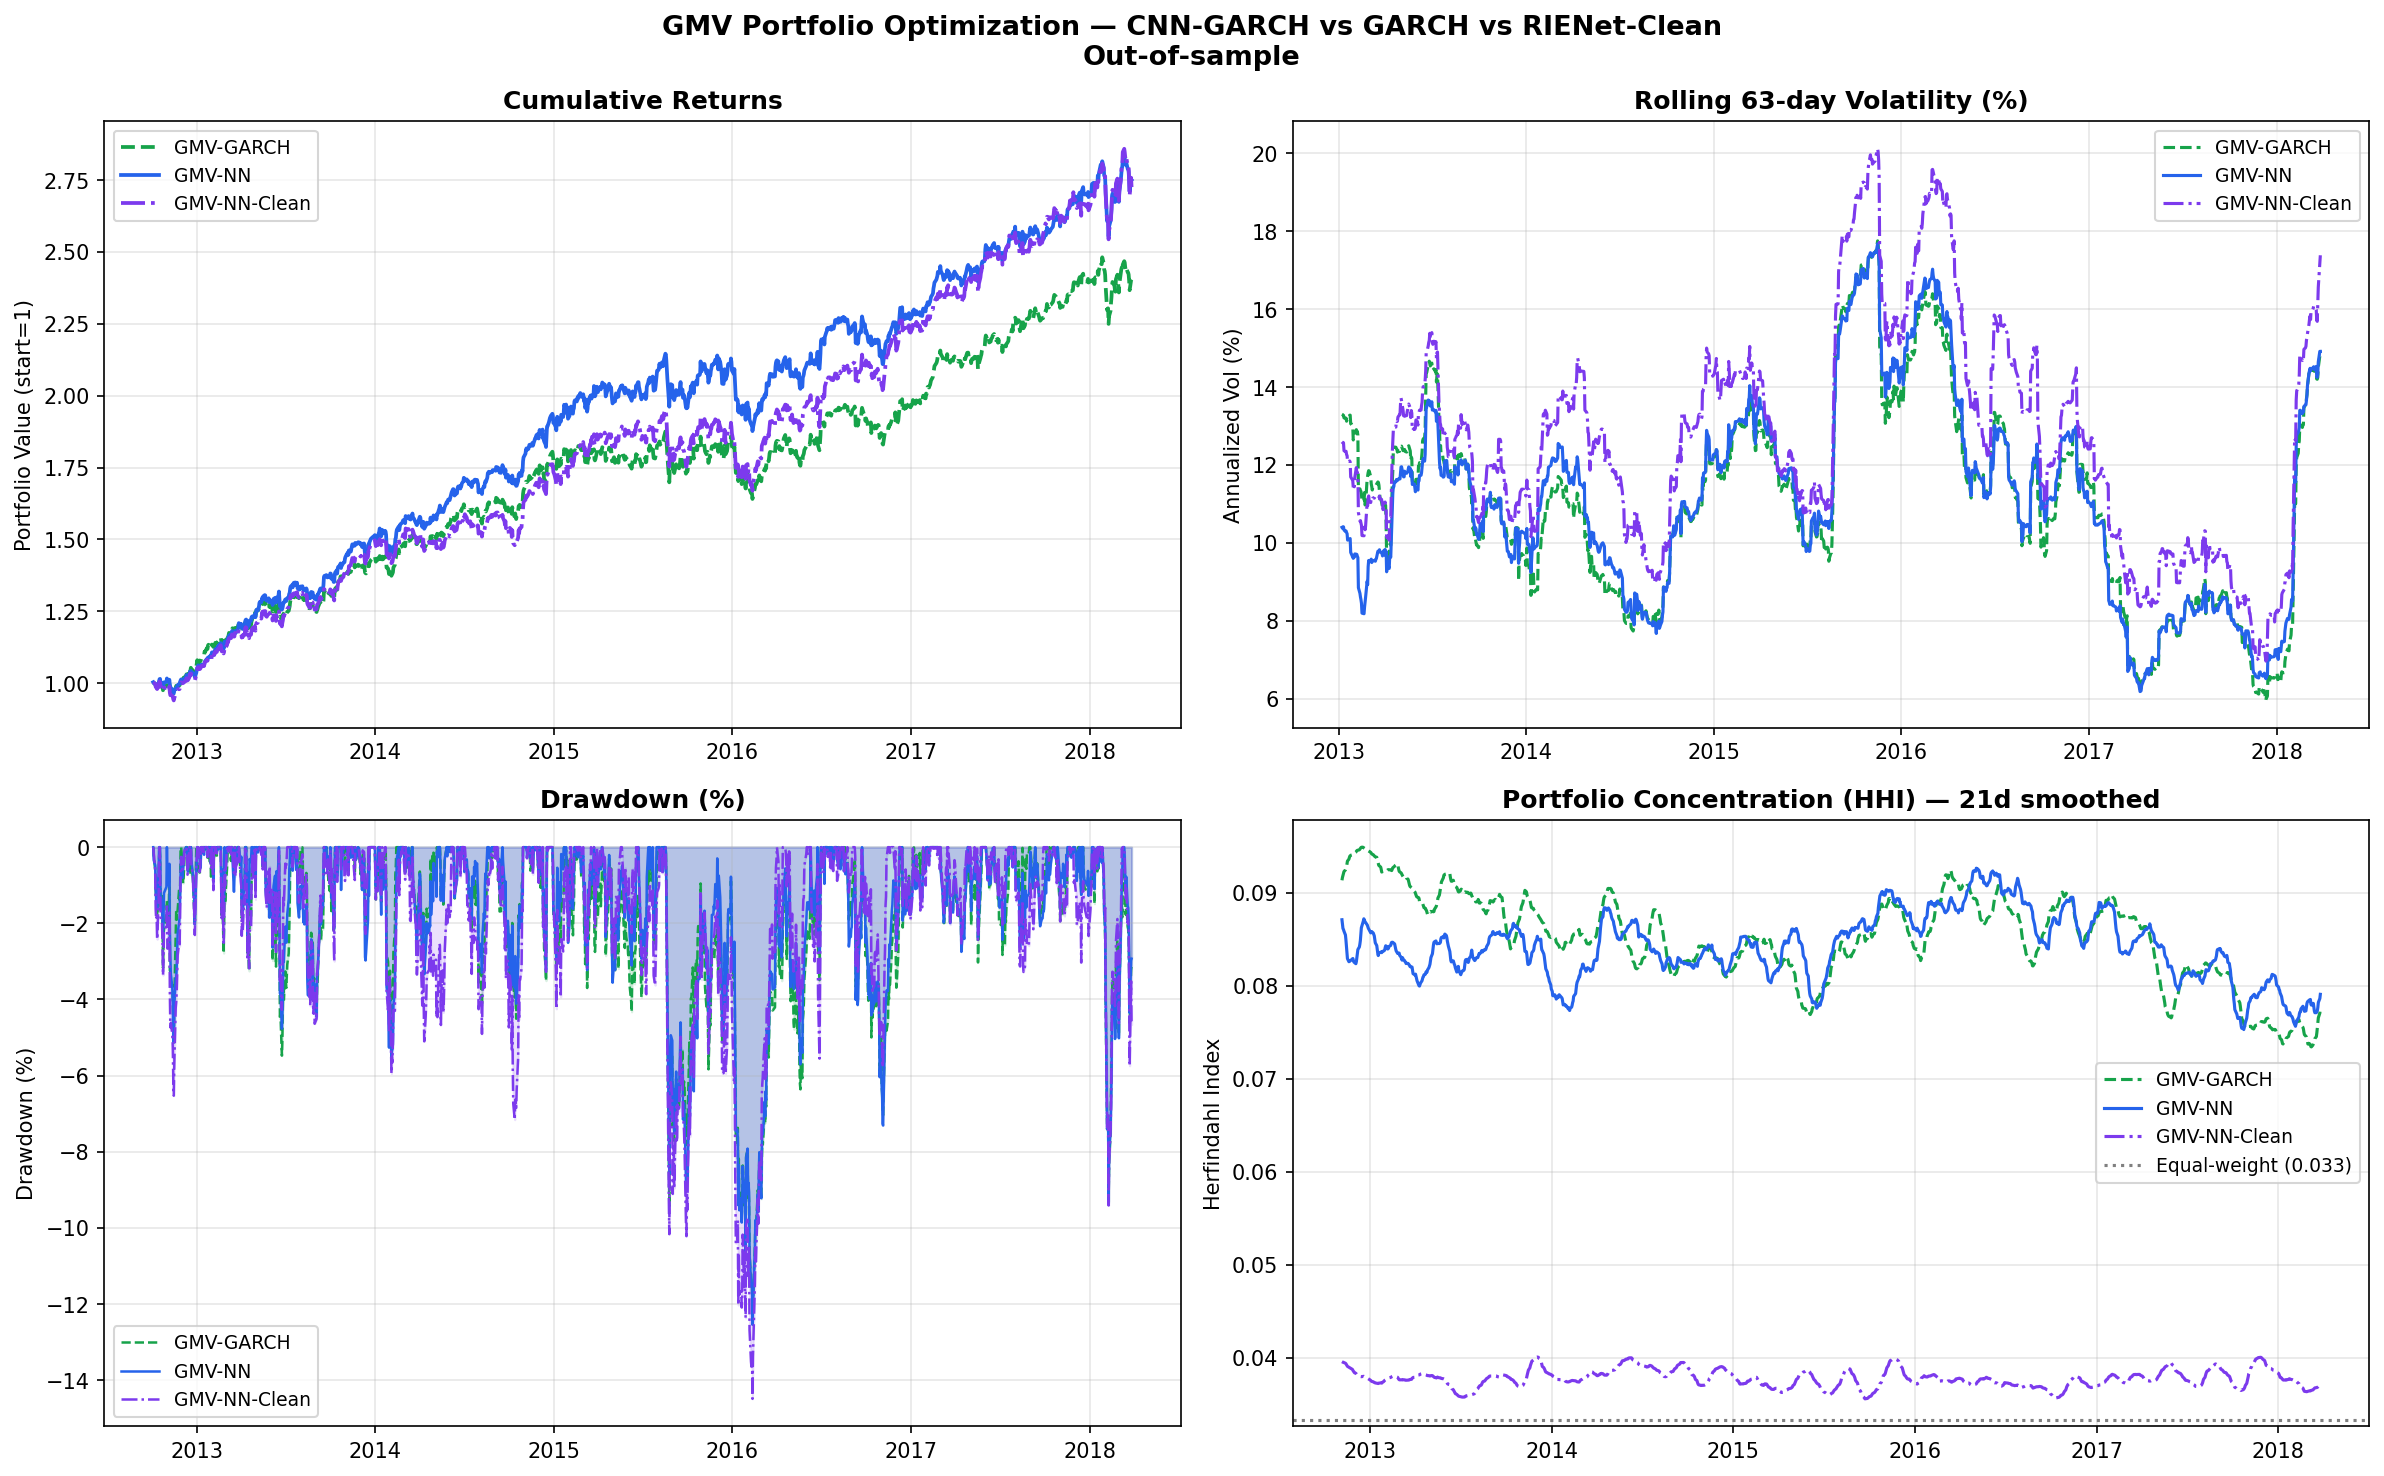
\includegraphics[width=0.84\textwidth]{gmv_results.png}
\caption{Example cumulative comparison from the constrained GMV experiments.}
\label{fig:gmv-constrained}
\end{figure}

\subsection{Monte Carlo robustness}

The Monte Carlo analysis in \texttt{Portfolio.ipynb} repeats the evaluation over 200 random selections of 30 stocks from the 1338-stock universe. This gives a better view of how stable the conclusions are beyond a single stock subset. The reported averages are:
\begin{itemize}[leftmargin=1.5em]
\item mean annualized volatility: 12.7555 for NN versus 13.1485 for ARCH/GARCH baseline;
\item mean Sharpe ratio: 1.1967 for NN versus 1.1525 for the baseline;
\item mean paired volatility gain: +0.3930;
\item mean paired Sharpe gain: +0.0442.
\end{itemize}

The paired Wilcoxon tests are strongly significant:
\begin{itemize}[leftmargin=1.5em]
\item volatility comparison: $W = 19563.0$, $p = 1.8875 \times 10^{-31}$;
\item Sharpe comparison: $W = 14172.0$, $p = 2.4582 \times 10^{-7}$.
\end{itemize}

These results support the claim that the neural model improves the volatility side of the portfolio problem in a statistically meaningful way over repeated resampling experiments.

\begin{figure}[H]
\centering
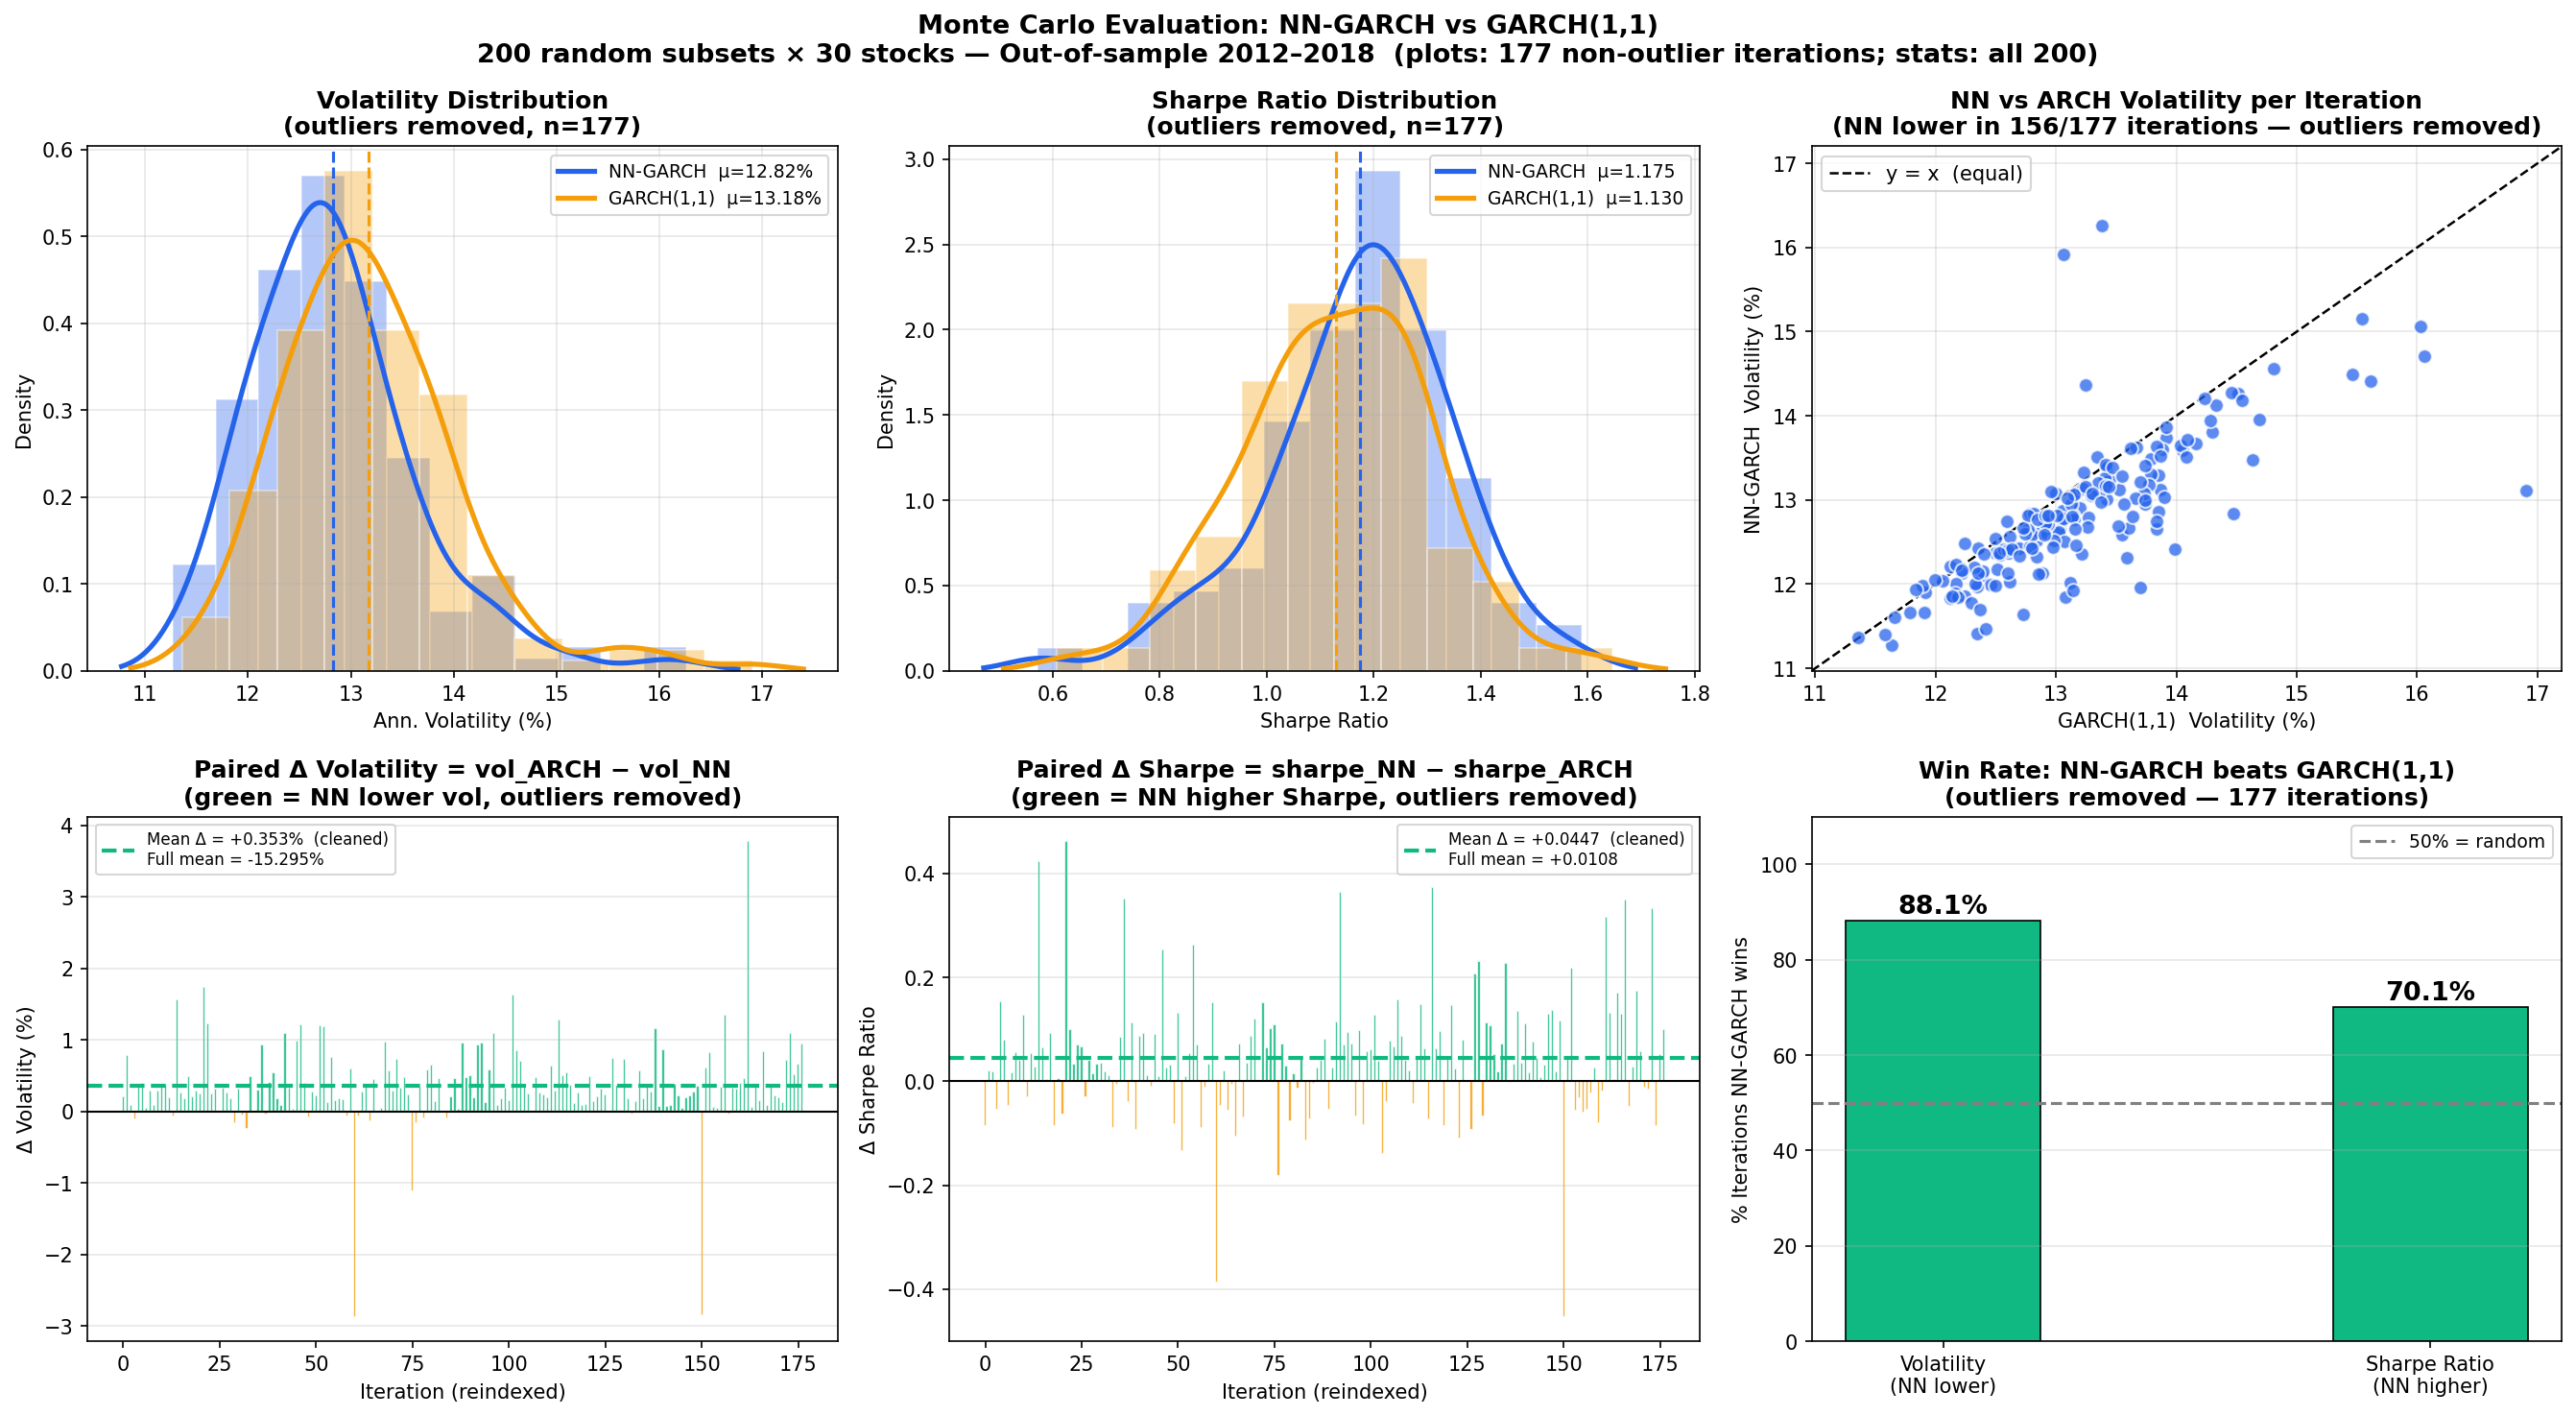
\includegraphics[width=0.78\textwidth]{mc_wilcoxon_distributions.png}
\caption{Monte Carlo distributions used for the paired Wilcoxon robustness study.}
\label{fig:wilcoxon}
\end{figure}

\subsection{Computational resources and cost}

The notebooks report CPU runtimes for the main experiments. In the 50-stock unconstrained notebook, volatility precomputation takes about 70.6 seconds for CNN-GARCH and 1.8 seconds for the benchmark GARCH recursion. In the constrained 30-stock notebook, the corresponding numbers are about 66.1 seconds and 0.6 seconds. In the 100-stock notebook, the CNN-GARCH pass takes about 114.9 seconds and the GARCH recursion about 4.9 seconds. The 200-run Monte Carlo study takes about 42.3 minutes on CPU.

These numbers show a clear trade-off. The neural model is slower than the benchmark, but the computational burden remains realistic for an academic daily-frequency pipeline. Monetary cost was not tracked because the experiments were run locally rather than through paid cloud infrastructure. If required for the final submission, the hardware description can be added here: \texttt{[fill local CPU / RAM / OS]}.

\section{Ethical and Societal Impact}

Although this project is primarily methodological, it still raises nontrivial ethical and practical issues. First, backtest success does not guarantee future reliability. Risk models trained on historical equity data can fail under regime changes, crises, or structural breaks. A model that looks safer than a benchmark in-sample or in one historical backtest can still fail when liquidity vanishes or correlations spike.

Second, unconstrained or weakly constrained variance-minimization portfolios may produce short positions and concentrated exposures that are unacceptable in real mandates. This matters especially when leverage is considered, because small covariance errors can translate into large capital allocations. The model should therefore be seen as a decision-support tool for research, not as a fully autonomous trading system ready for deployment.

Third, the data pipeline may still contain survivorship, delisting, or stale-price effects despite the cleaning rules. Daily data also understate intraday liquidity stress and trading frictions. A socially responsible presentation of the project should therefore state clearly that transaction costs, market impact, and operational constraints are not yet fully modeled.

\section{Project Organization}

This section should be finalized with the exact division of labor agreed by the team before submission. A report is stronger when it documents not only the final model, but also how the project was organized over time.

\subsection{Task distribution draft}

\begin{table}[H]
\centering
\caption{Draft template for task distribution. Replace the placeholders with the exact final split.}
\label{tab:task-distribution}
\begin{tabularx}{\textwidth}{lXX}
\toprule
Task & Main responsibility & Notes \\
\midrule
Literature review and state of the art & [fill] & Bongiorno papers, GARCH, covariance cleaning, hybrid NN literature \\
Data cleaning and preprocessing & [fill] & WIKI panel cleaning, asset filters, train/test split \\
Synthetic pretraining & [fill] & Simulated GARCH data generation and first model fit \\
Real-data fine-tuning & [fill] & Zero-aware filtering, validation checkpoints, diagnostics \\
Portfolio evaluation & [fill] & GMV experiments, constrained/unconstrained comparisons, robustness \\
Poster and report writing & [fill] & Slides, poster, tables, final narrative \\
\bottomrule
\end{tabularx}
\end{table}

\subsection{Time spent draft}

\begin{table}[H]
\centering
\caption{Editable hours table.}
\label{tab:hours}
\begin{tabular}{lccc}
\toprule
Task & Wacil (h) & Sneha (h) & Total (h) \\
\midrule
Reading and planning & [fill] & [fill] & [fill] \\
Implementation and debugging & [fill] & [fill] & [fill] \\
Training and experimentation & [fill] & [fill] & [fill] \\
Evaluation and figure production & [fill] & [fill] & [fill] \\
Writing and presentation & [fill] & [fill] & [fill] \\
\midrule
Total & [fill] & [fill] & [fill] \\
\bottomrule
\end{tabular}
\end{table}

\subsection{Timeline draft}

\begin{table}[H]
\centering
\caption{Simple Gantt-style timeline for the report.}
\label{tab:timeline}
\begin{tabularx}{\textwidth}{lXXXXX}
\toprule
Work package & Week 1 & Week 2 & Week 3 & Week 4 & Week 5 \\
\midrule
Problem definition and reading & X & X &  &  &  \\
Data pipeline and cleaning &  & X & X &  &  \\
Synthetic pretraining &  & X & X &  &  \\
Real-data fine-tuning &  &  & X & X &  \\
Portfolio experiments &  &  &  & X & X \\
Poster and report preparation &  &  &  & X & X \\
\bottomrule
\end{tabularx}
\end{table}

\section{Conclusion and Perspectives}

The project starts from a simple observation: GMV portfolios are mostly limited by covariance estimation error rather than by the closed-form optimizer itself. This is why GARCH is an appropriate benchmark, and also why a hybrid neural extension is worth testing. The experiments show that the CNN-GARCH model improves the volatility-estimation stage in several relevant settings, and that correlation cleaning can further reduce portfolio risk in the main 50-stock unconstrained experiment.

The most careful conclusion is therefore the following. The project does not prove that the GMV estimation problem is fully solved. It does show that better marginal volatility forecasts and better-conditioned correlation estimates can materially improve out-of-sample portfolio behavior. In the main result, GMV-NN-Clean delivers the lowest volatility, while GMV-NN delivers the highest Sharpe ratio. This is exactly the kind of nuanced outcome that should be reported honestly.

The next steps are clear: add transaction costs and turnover penalties, test stricter long-only constraints, compare against shrinkage and risk-parity baselines, scale to larger universes, and explore tighter joint training between the volatility and covariance-cleaning modules. A stronger study could also include crisis-period stress tests and more detailed hardware-cost reporting.

\begin{thebibliography}{99}

\bibitem{markowitz1952}
H. Markowitz.
\newblock Portfolio selection.
\newblock \emph{The Journal of Finance}, 7(1):77--91, 1952.

\bibitem{engle1982}
R. F. Engle.
\newblock Autoregressive conditional heteroscedasticity with estimates of the variance of United Kingdom inflation.
\newblock \emph{Econometrica}, 50(4):987--1007, 1982.

\bibitem{bollerslev1986}
T. Bollerslev.
\newblock Generalized autoregressive conditional heteroskedasticity.
\newblock \emph{Journal of Econometrics}, 31(3):307--327, 1986.

\bibitem{ledoit2004}
O. Ledoit and M. Wolf.
\newblock A well-conditioned estimator for large-dimensional covariance matrices.
\newblock \emph{Journal of Multivariate Analysis}, 88(2):365--411, 2004.

\bibitem{bongiorno2025e2e}
C. Bongiorno, E. Manolakis, and R. N. Mantegna.
\newblock End-to-end large portfolio optimization for variance minimization with neural networks through covariance cleaning.
\newblock Working paper / conference manuscript, 2025.

\bibitem{bongiorno2025icaif}
C. Bongiorno, E. Manolakis, and R. N. Mantegna.
\newblock Neural network-driven volatility drag mitigation under aggressive leverage.
\newblock Working paper / ICAIF manuscript, 2025.

\bibitem{michankow2023}
J. Micha\'nk\'ow, L. Kwiatkowski, and J. Morajda.
\newblock Combining deep learning and GARCH models for financial volatility and risk forecasting.
\newblock \emph{arXiv preprint arXiv:2310.01063}, 2023.

\bibitem{wang2025}
H. Wang, C. Liu, M.-N. Tran, and C. Wang.
\newblock Deep learning enhanced multivariate GARCH.
\newblock \emph{arXiv preprint arXiv:2506.02796}, 2025.

\end{thebibliography}

\end{document}
